% interactcadsample.tex
% v1.03 - April 2017

\documentclass[]{interact}

\usepackage{epstopdf}% To incorporate .eps illustrations using PDFLaTeX, etc.
\usepackage{subfigure}% Support for small, `sub' figures and tables
%\usepackage[nolists,tablesfirst]{endfloat}% To `separate' figures and tables from text if required

\usepackage{natbib}% Citation support using natbib.sty
\bibpunct[, ]{(}{)}{;}{a}{}{,}% Citation support using natbib.sty
\renewcommand\bibfont{\fontsize{10}{12}\selectfont}% Bibliography support using natbib.sty

\theoremstyle{plain}% Theorem-like structures provided by amsthm.sty
\newtheorem{theorem}{Theorem}[section]
\newtheorem{lemma}[theorem]{Lemma}
\newtheorem{corollary}[theorem]{Corollary}
\newtheorem{proposition}[theorem]{Proposition}

\theoremstyle{definition}
\newtheorem{definition}[theorem]{Definition}
\newtheorem{example}[theorem]{Example}

\theoremstyle{remark}
\newtheorem{remark}{Remark}
\newtheorem{notation}{Notation}

% see https://stackoverflow.com/a/47122900

% Pandoc citation processing

\usepackage{hyperref}
\usepackage[utf8]{inputenc}
\def\tightlist{}


\begin{document}

\articletype{ORIGINAL RESEARCH ARTICLE}

\title{Morphological trajectories suggest significant changes in
preference and design intent associated with Gahagan bifaces from Caddo
burials in the American Southeast}


\author{\name{Robert Z. Selden, Jr.$^{a}$, John E. Dockall$^{b}$}
\affil{$^{a}$Heritage Research Center, Stephen F. Austin State
University; Department of Biology, Stephen F. Austin State University;
Cultural Heritage Department, Jean Monnet
University; $^{b}$Cox\textbar McClain Environmental Consultants, Inc.}
}

\thanks{CONTACT Robert Z. Selden,
Jr.. Email: \href{mailto:zselden@sfasu.edu}{\nolinkurl{zselden@sfasu.edu}}, John
E.
Dockall. Email: \href{mailto:johnd@coxmcclain.com}{\nolinkurl{johnd@coxmcclain.com}}}

\maketitle

\begin{abstract}
Gahagan bifaces differ in morphology across the same geography as Caddo
bottles and Perdiz arrow points, and also between the Caddo and central
Texas regions. This study asks whether Gahagan biface morphology differs
between stratigraphically-defined---and chronologically
discrete---burial contexts at the Mounds Plantation and George C. Davis
sites, and whether Gahagan biface morphology may differ based on
qualitative differences in Caddo burial practices. Results indicate a
significant difference in size between burial contexts at Mounds
Plantation and George C. Davis, where the pattern is inverted. At both
sites, biface shape remains consistent and does not differ among
contexts, indicating an established \texttt{shape\ preference} in the
northern and southern behavioral regions that may have shifted
significantly in size due to cyclical differences in the variable social
mechanisms associated with raw material procurement. Gahagan bifaces
also differ in shape between Caddo burial contexts where a biface was
placed \emph{alongside an individual} and those found as part of a cache
placed \emph{alongside the northern wall of the burial feature}. Each
burial tradition articulates with a distinct
\texttt{community\ of\ practice} relating to Gahagan biface
\texttt{placement} and \texttt{design\ intent}.
\end{abstract}

\begin{keywords}
Caddo; NAGPRA; archaeoinformatics; 3D geometric morphometrics; museum
studies; digital humanities
\end{keywords}

\hypertarget{introduction}{%
\section{Introduction}\label{introduction}}

Found to occur along the western margin of the American Southeast,
Gahagan bifaces are among the most recognizable and well known
components of Caddo material culture, and were regularly included with
burial offerings during the Formative (CE 800-1000) and Early (CE
1000-1250) Caddo periods
\citep{RN7115,RN8189,RN5746,RN8186,RN8174,RN8176}. Recent efforts to
characterize general trends associated with Gahagan biface morphology
yielded support for a \texttt{spatial\ boundary} that divides the
northern and southern Caddo behavioral regions based upon morphological
differences that occur in Caddo bottles, Gahagan bifaces, and Perdiz
arrow points (Figure 1c)
\citep{RN7925,RN8071,RN8361,RN8967,RN11064,RN8154}. A second
\texttt{shape\ boundary} has also been posited based upon differences in
Gahagan biface morphology between the Caddo and central Texas regions
\citep{RN8318}.

\begin{figure}
\includegraphics[width=1\linewidth]{img/fig01} \caption{Mean shapes and comparisons for a, Formative/Early (Selden Jr. 2018a,b, 2019) and b, Late/Historic bottles (Selden Jr. 2021); c, Formative/Early Gahagan bifaces (Selden Jr., Dockall, and Shafer 2018, Selden Jr., Dockall, and Dubied 2020); and d, Middle/Late Perdiz arrow points from Caddo burial contexts in the northern and southern behavioral regions (Selden and Dockall 2021). In the comparisons of mean shape, the northern population appears in gray, and the southern population appears in black.}\label{fig:fig01}
\end{figure}

\hypertarget{contexts-of-recovery}{%
\section{Contexts of recovery}\label{contexts-of-recovery}}

All Gahagan bifaces used in this analysis were recovered from Caddo
burial contexts, and were excavated between 1912 and 1969. Stratigraphic
contexts were used to delimit temporal contexts---although the span of
that temporal difference remains unclear---and figures were redrafted
from the original works that illustrate clear stratigraphic differences.
Additional contextual information was used to identify Gahagan bifaces
placed atop or alongside an individual, or in caches along the northern
wall of the burial pit. Specific references are made to published images
and illustrations that depict these burial contexts during excavation.
While no images or illustrations of burial contexts were included here,
those are included with the supplemental materials \citep{RN11065}.

\hypertarget{gahagan-mound}{%
\subsection{Gahagan Mound}\label{gahagan-mound}}

Gahagan bifaces were identified in 1911 in Deposits 1, 2, and 3 of
Burial Pit 1 at the Gahagan Mound site in northwest Louisiana by
\citet[Figures 18-19, 21]{RN7115}. A subsequent excavation at the
Gahagan Mound site in 1936 identified two additional burial features
containing Gahagan bifaces (Burial Pits 2 and 3) (Figure 2)
\citep[Plate 27]{RN8176}, and the entirety of the Gahagan Mound site was
eventually destroyed by the meander of the Red River between four and
five years later \citep{RN10759}.

\hypertarget{mounds-plantation}{%
\subsection{Mounds Plantation}\label{mounds-plantation}}

\hypertarget{george-c.-davis}{%
\subsection{George C. Davis}\label{george-c.-davis}}

\begin{figure}
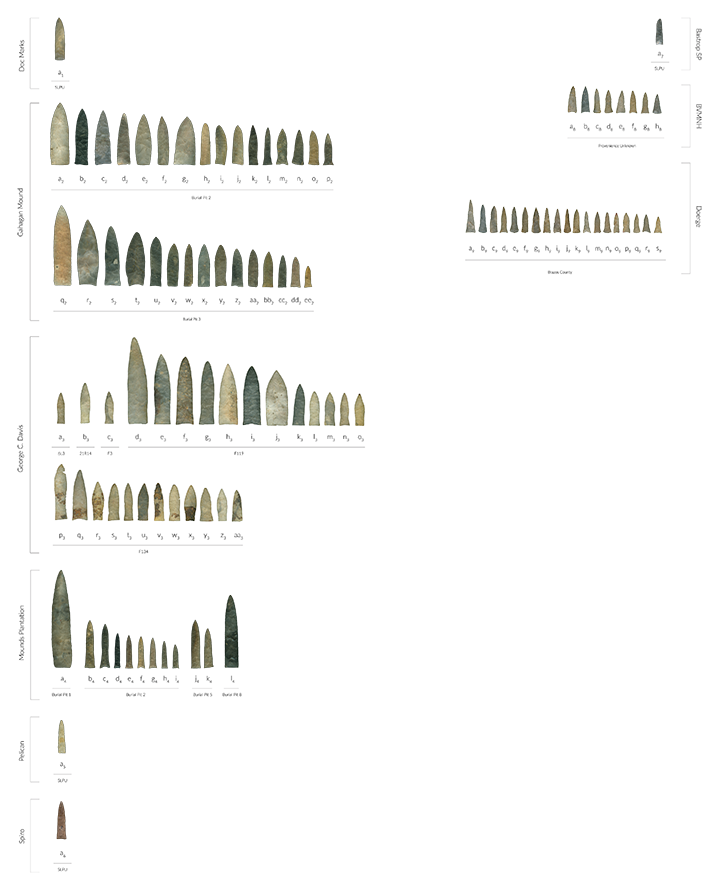
\includegraphics[width=0.85\linewidth]{img/fig02} \caption{Gahagan bifaces from the northern and southern Caddo behavioral regions. Bifaces recovered atop or alongside an individual denoted by black dot. As a reference to scale, the Gahagan biface at bottom left (m3) measures 48cm in length. Additional information for each biface, including the option to download full-resolution 2D images of individual bifaces, can be found at https://scholarworks.sfasu.edu/ita-gahaganbiface/.}\label{fig:gahagan bifaces 2D}
\end{figure}

\hypertarget{associated-diagnostics}{%
\section{Associated diagnostics}\label{associated-diagnostics}}

\begin{figure}
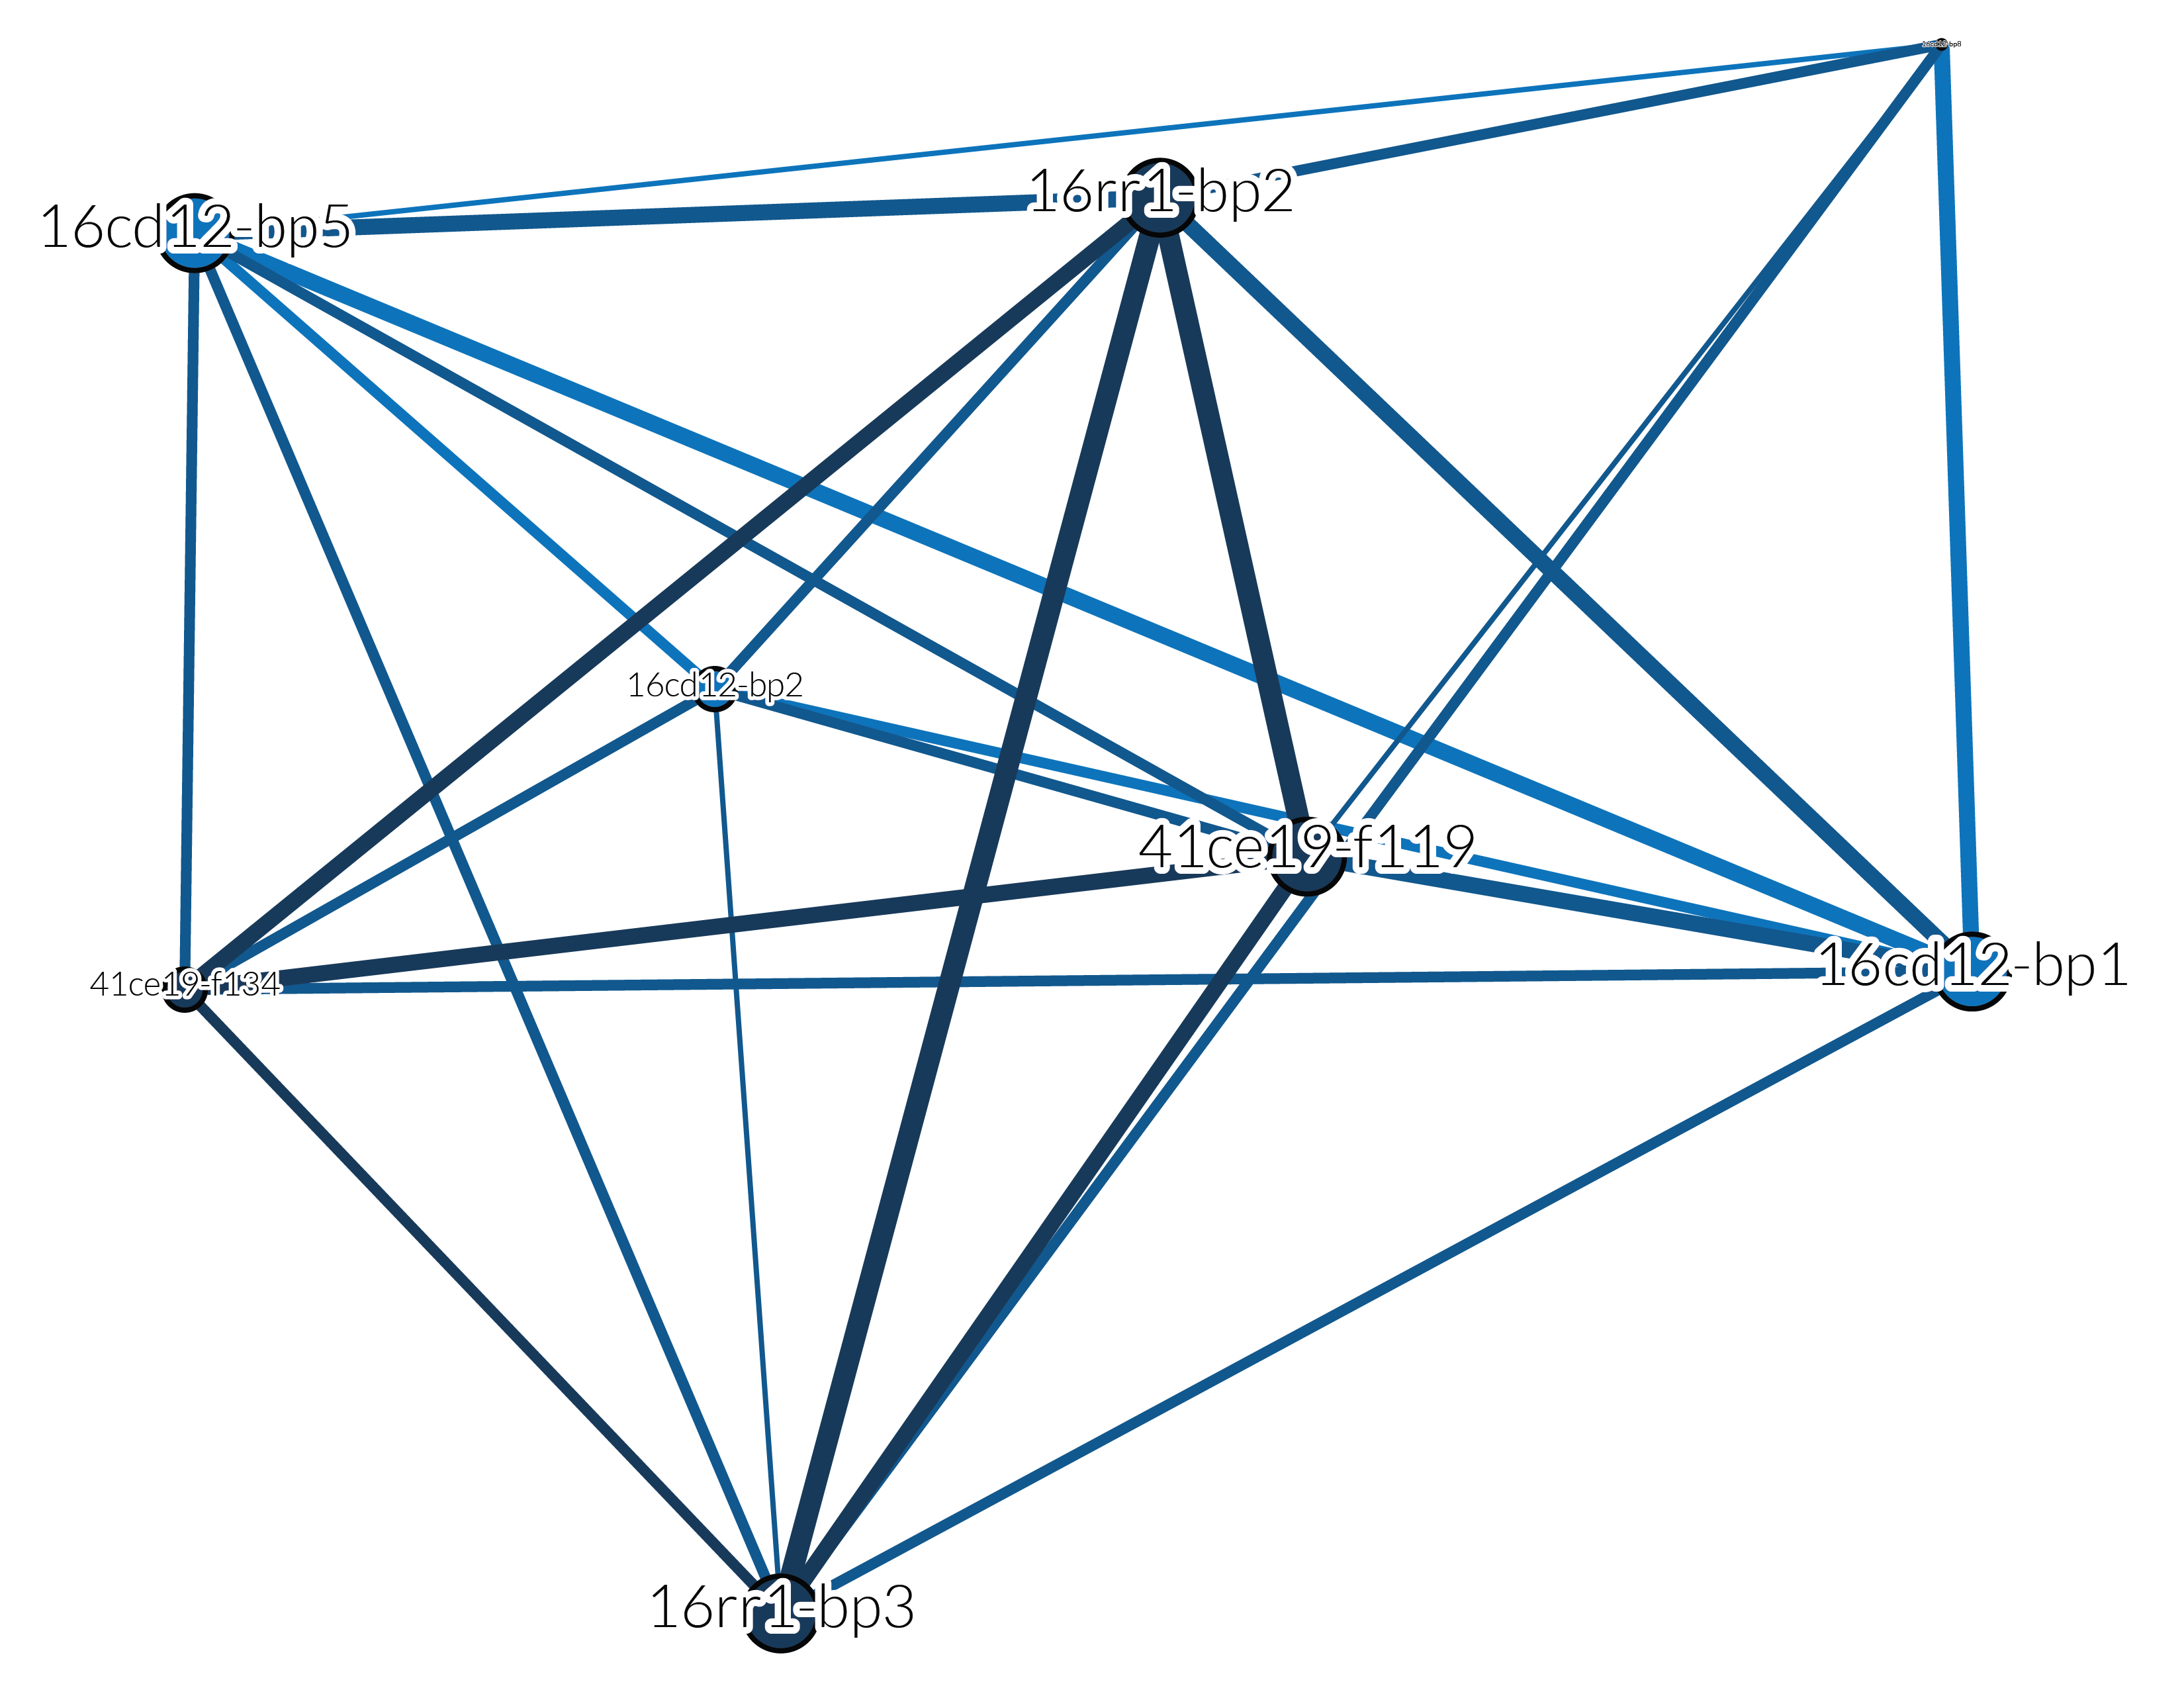
\includegraphics[width=1\linewidth]{img/fig03} \caption{Network of associated diagnostic artifacts recovered with Gahagan bifaces. The thicker and darker the line between contexts, the larger the number of co-present diagnostic artifacts.}\label{fig:associated.net}
\end{figure}

\begin{table}
\tbl{Diagnostic artifact types from Caddo burials found in association with Gahagan bifaces.}
{\begin{tabular}{ll} \toprule
Contexts & Diagnostics \\
\midrule
16CD12-BP1 & AL, CA, CC, FR, HA, HE, HFE \\
16CD12-BP2 & AL, HA \\
16CD12-BP5 & AL, FR, HA, SC \\
16CD12-BP8 & CA, HE, HFE, SC \\
16RR1-BP2 & AL, C, HA, HFE, HR, KI, SC \\
16RR1-BP3 & AL, C, HFE, SC \\
41CE19-F119 & AL, C, HA, HFE \\
41CE19-F134 & AL, C, HA \\
\bottomrule
\end{tabular}}
\tabnote{Associated diagnostic artifacts from Caddo burial contexts at the Mounds Plantation (16CD12), Gahagan Mound (16RR1), and George C. Davis (41CE19) sites include Alba arrow points (AL), celts (C), Catahoula arrow points (CA), Coles Creek ceramics (CC), Friley arrow points (FR), Gahagan bifaces (GB), Hayes arrow points (HA), Hickory Engraved ceramics (HE), Holly Fine Engraved ceramics (HFE), Harrell arrow points (HR), Kiam Incised ceramics (KI), and Scallorn arrow points (SC).}
\label{sample-table}
\end{table}

\hypertarget{methods}{%
\section{Methods}\label{methods}}

\hypertarget{discussion-and-conclusion}{%
\section{Discussion and Conclusion}\label{discussion-and-conclusion}}

\hypertarget{acknowledgments}{%
\section*{Acknowledgments}\label{acknowledgments}}
\addcontentsline{toc}{section}{Acknowledgments}

We extend our gratitude to the Caddo Nation of Oklahoma, the Williamson
Museum at Northwestern State University, the Louisiana State Exhibit
Museum, the Texas Archeological Research Laboratory at The University of
Texas at Austin, the Brazos Valley Museum of Natural History, the Texas
Parks and Wildlife Department, and the Sam Noble Oklahoma Museum of
Natural Science for the requisite permissions and access needed to
generate 3D scans of the Gahagan bifaces. Thanks to Harry J. Shafer,
Hiram F. (Pete) Gregory, Christian S. Hoggard, and David K. Thulman for
their comments on the analyses of Gahagan biface shape.

RZS extends his gratitude to Christian S. Hoggard and David K. Thulman
for their thoughtful comments and constructive criticisms of the
landmarking protocol used in this study
(\href{https://github.com/aksel-blaise/gahaganmorph2/blob/master/analysis/landmarking-protocol.md}{\texttt{LM3d1}}),
as well as the landmarking protocol for Gahagan bifaces that will be
used in the next iteration of these analytical efforts
(\href{https://seldenlab.github.io/gahaganmorph.3/landmarking-protocol-3d2.html}{\texttt{LM3d2}});
to Martin Hinz for fielding questions related to the \texttt{oxcAAR}
package and Derek Hamilton for his guidance with the chronological
models; and to Dean C. Adams, Michael L. Collyer, Emma Sherratt, Lauren
Butaric, and Kersten Bergstrom for their constructive criticisms,
general comments, and suggestions throughout the development of this
research program.

\hypertarget{funding}{%
\section*{Funding}\label{funding}}
\addcontentsline{toc}{section}{Funding}

Components of this analytical work flow were developed and funded by a
Preservation Technology and Training grant (P14AP00138) to RZS from the
National Center for Preservation Technology and Training (NCPTT), and
additional grants to RZS from the Caddo Nation of Oklahoma, National
Forests and Grasslands in Texas (15-PA-11081300-033) and the United
States Forest Service (20-PA-11081300-074). Funding to scan the Gahagan
bifaces at the Williamson Museum at Northwestern State University,
Louisiana State Exhibit Museum, Texas Archeological Research Laboratory
at The University of Texas at Austin, and Sam Noble Oklahoma Museum of
Natural Science was provided to the RZS by the Heritage Research Center
at Stephen F. Austin State University.

\hypertarget{data-management}{%
\section*{Data management}\label{data-management}}
\addcontentsline{toc}{section}{Data management}

The analysis code associated with this project can be accessed through
this document or the
\href{https://github.com/seldenlab/gahaganmorph.3}{GitHub} repository,
which is digitally curated on the Open Science Framework
\href{https://osf.io/y7b39/}{DOI: 10.17605/OSF.IO/Y7B39}. The
reproducible nature of this undertaking provides a means for others to
critically assess and evaluate the various analytical components
\citep{RN8312,RN8313,RN8299}, which is a necessary requirement for the
production of reliable knowledge.

Reproducibility projects in \href{https://osf.io/ezcuj/}{psychology} and
\href{https://www.cos.io/rpcb}{cancer biology} are impacting current
research practices across all domains. Examples of reproducible research
are becoming more abundant in archaeology
\citep{RN8207,RN8965,RN8154,RN8318,RN9364}, and the next generation of
archaeologists are learning those tools and methods needed to reproduce
and/or replicate research results \citep{RN10760}. Reproducible and
replicable research work flows are often employed at the highest levels
of humanities-based inquiries to mitigate concern or doubt regarding
proper execution, and is of particular import should the results
have---explicitly or implicitly---a major impact on scientific progress
\citep{RN10761}.

\bibliographystyle{tfcad}
\bibliography{interactcadsample.bib}


\input{"appendix.tex"}


\end{document}
